\documentclass[tikz,border=3mm]{standalone}
\usepackage[T1]{fontenc}
\usepackage{lmodern}
\usepackage{amsmath,amssymb}
\usepackage{tikz}
\usetikzlibrary{arrows.meta,calc,fit,positioning,shapes.geometric,backgrounds}

\definecolor{ink}{HTML}{173041}
\definecolor{muted}{HTML}{667982}
\definecolor{green}{HTML}{08705B}
\definecolor{greenlite}{HTML}{E6F4EE}
\definecolor{blue}{HTML}{285F94}
\definecolor{bluelite}{HTML}{E9F0F8}
\definecolor{orange}{HTML}{A86522}
\definecolor{orangelite}{HTML}{FFF2DF}
\definecolor{line}{HTML}{CFDBD7}
\definecolor{paper}{HTML}{F7FAF9}

\tikzset{
  font=\sffamily,
  panel/.style={draw=line,fill=white,rounded corners=2mm,line width=.35pt},
  heading/.style={font=\sffamily\bfseries\small,text=ink},
  note/.style={font=\sffamily\scriptsize,text=muted},
  flow/.style={-{Latex[length=2.2mm]},line width=.55pt,draw=muted},
  neuronI/.style={circle,draw=green,fill=greenlite,minimum size=2.2mm,inner sep=0pt},
  neuronE/.style={circle,draw=blue,fill=bluelite,minimum size=2.2mm,inner sep=0pt},
  loss/.style={draw=line,fill=paper,rounded corners=1.4mm,inner sep=2.2mm,align=left},
  sampleI/.style={circle,fill=green,minimum size=.8mm,inner sep=0pt},
  sampleE/.style={circle,fill=blue,minimum size=.8mm,inner sep=0pt},
  sampleG/.style={circle,fill=orange,minimum size=1.05mm,inner sep=0pt}
}

\begin{document}
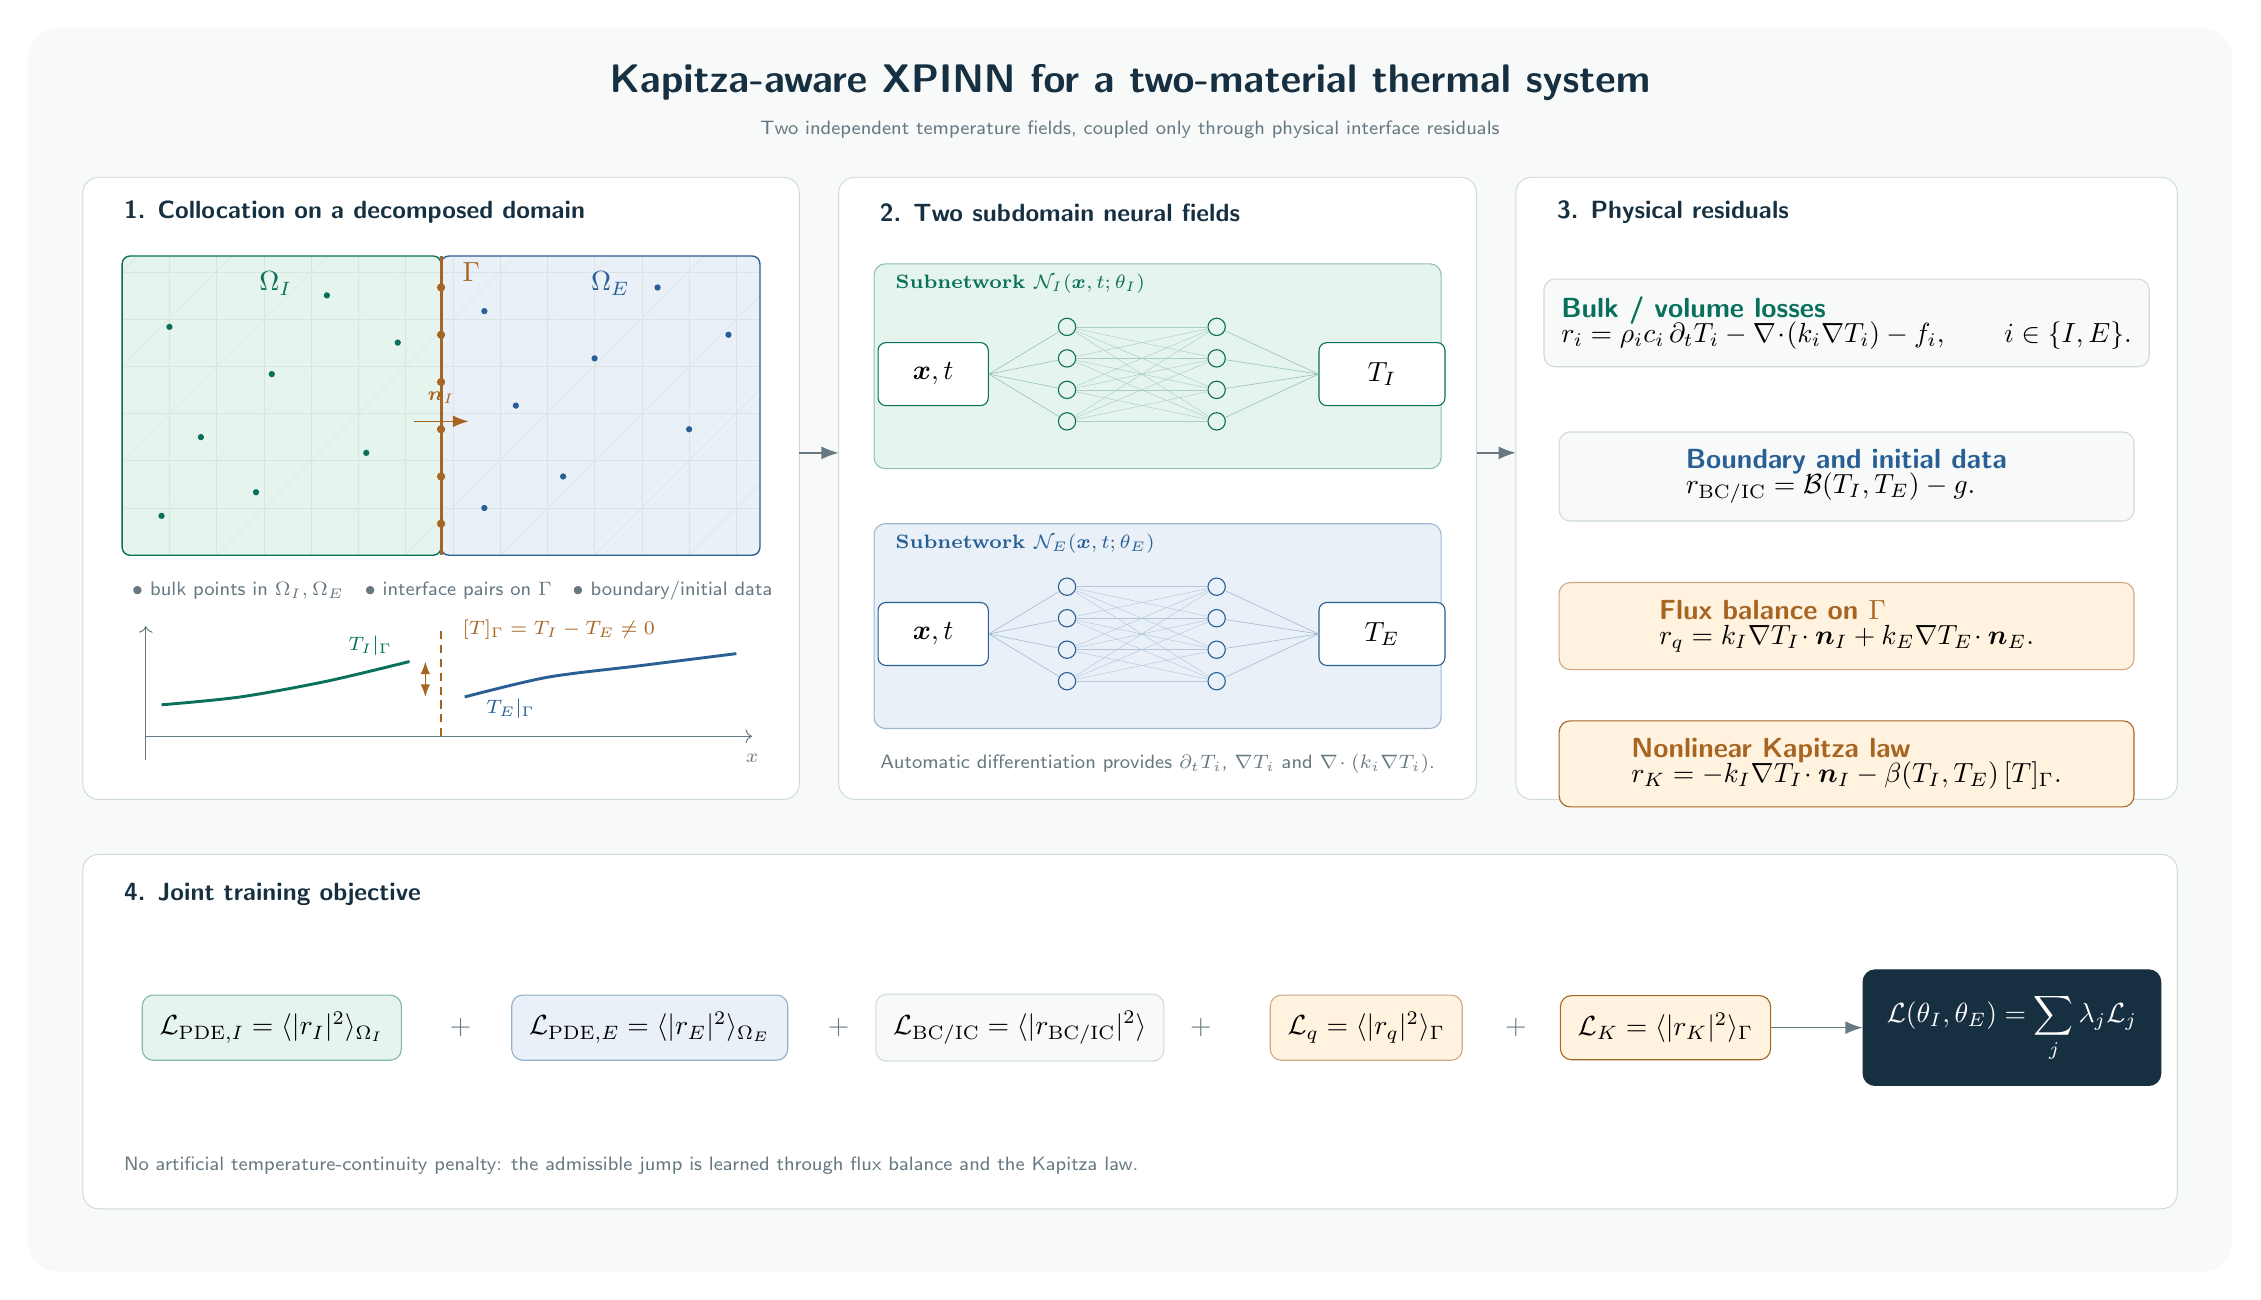
\begin{tikzpicture}[x=1mm,y=1mm]
  \fill[paper,rounded corners=4mm] (0,0) rectangle (280,158);
  \node[font=\sffamily\bfseries\Large,text=ink] at (140,151)
    {Kapitza-aware XPINN for a two-material thermal system};
  \node[note] at (140,145)
    {Two independent temperature fields, coupled only through physical interface residuals};

  % ------------------------------------------------------------------
  % Panel A: a large, fully sampled 2-D composite domain
  \path[panel] (7,60) rectangle (98,139);
  \node[heading,anchor=west] at (11,134.5) {1. Collocation on a decomposed domain};
  \begin{scope}
    \clip[rounded corners=1mm] (12,91) rectangle (93,129);
    \fill[greenlite] (12,91) rectangle (52.5,129);
    \fill[bluelite] (52.5,91) rectangle (93,129);
    % structured background mesh
    \foreach \x in {18,24,...,90}{\draw[line!75,line width=.18pt] (\x,91)--(\x,129);}
    \foreach \y in {97,103,...,127}{\draw[line!75,line width=.18pt] (12,\y)--(93,\y);}
    \foreach \x in {12,24,...,84}{
      \foreach \y in {91,103,...,127}{\draw[line!75,line width=.18pt] (\x,\y)--++(12,12);}
    }
    % collocation clouds
    \foreach \x/\y in {17/96,22/106,18/120,29/99,31/114,38/124,43/104,47/118}
      \node[sampleI] at (\x,\y) {};
    \foreach \x/\y in {58/97,62/110,58/122,68/101,72/116,80/125,84/107,89/119}
      \node[sampleE] at (\x,\y) {};
  \end{scope}
  \draw[green,line width=.5pt,rounded corners=1mm] (12,91) rectangle (52.5,129);
  \draw[blue,line width=.5pt,rounded corners=1mm] (52.5,91) rectangle (93,129);
  \draw[orange,line width=1.1pt] (52.5,91)--(52.5,129);
  \foreach \y in {95,101,...,125}{\node[sampleG] at (52.5,\y) {};}
  \node[text=green] at (31.5,125.5) {$\Omega_I$};
  \node[text=blue] at (74,125.5) {$\Omega_E$};
  \node[text=orange,anchor=west] at (54,127) {$\Gamma$};
  \draw[-{Latex[length=2mm]},orange,line width=.6pt] (49,108)--(56,108)
    node[midway,above=1mm,font=\scriptsize,text=orange] {$\boldsymbol n_I$};
  \node[note,align=left,anchor=west] at (12,86.5)
    {$\bullet$ bulk points in $\Omega_I,\Omega_E$\quad
     $\bullet$ interface pairs on $\Gamma$\quad
     $\bullet$ boundary/initial data};

  % temperature jump plot directly below the domain
  \draw[->,muted,line width=.35pt] (15,65)--(15,82);
  \draw[->,muted,line width=.35pt] (15,68)--(92,68) node[below=1mm,note] {$x$};
  \draw[green,line width=1.05pt]
    plot[smooth] coordinates {(17,72) (27,73) (38,75) (48.5,77.5)};
  \draw[blue,line width=1.05pt]
    plot[smooth] coordinates {(55.5,73) (66,75.5) (78,77) (90,78.5)};
  \draw[orange,densely dashed,line width=.45pt] (52.5,68)--(52.5,82);
  \draw[orange,{Latex[length=1.6mm]}-{Latex[length=1.6mm]},line width=.5pt]
    (50.5,77.5)--(50.5,73);
  \node[font=\scriptsize,text=green,anchor=east] at (47.5,79.5) {$T_I|_{\Gamma}$};
  \node[font=\scriptsize,text=blue,anchor=west] at (57,71.5) {$T_E|_{\Gamma}$};
  \node[font=\scriptsize,text=orange,anchor=west] at (54,81.5)
    {$[T]_{\Gamma}=T_I-T_E\neq 0$};

  % ------------------------------------------------------------------
  % Panel B: neural approximation
  \path[panel] (103,60) rectangle (184,139);
  \node[heading,anchor=west] at (107,134.5) {2. Two subdomain neural fields};
  \node[loss,fill=greenlite,draw=green!45,minimum width=72mm,minimum height=26mm]
    (netI) at (143.5,115) {};
  \node[loss,fill=bluelite,draw=blue!45,minimum width=72mm,minimum height=26mm]
    (netE) at (143.5,82) {};
  \node[font=\bfseries\scriptsize,text=green,anchor=west] at (109,125.5) {Subnetwork $\mathcal N_I(\boldsymbol x,t;\theta_I)$};
  \node[font=\bfseries\scriptsize,text=blue,anchor=west] at (109,92.5) {Subnetwork $\mathcal N_E(\boldsymbol x,t;\theta_E)$};
  \node[draw=green,fill=white,rounded corners=1mm,minimum width=14mm,minimum height=8mm]
    (inI) at (115,114) {$\boldsymbol x,t$};
  \node[draw=green,fill=white,rounded corners=1mm,minimum width=16mm,minimum height=8mm]
    (outI) at (172,114) {$T_I$};
  \node[draw=blue,fill=white,rounded corners=1mm,minimum width=14mm,minimum height=8mm]
    (inE) at (115,81) {$\boldsymbol x,t$};
  \node[draw=blue,fill=white,rounded corners=1mm,minimum width=16mm,minimum height=8mm]
    (outE) at (172,81) {$T_E$};
  \foreach \yy in {108,112,116,120}{\node[neuronI] (ia\yy) at (132,\yy) {};\node[neuronI] (ib\yy) at (151,\yy) {};}
  \foreach \yy in {75,79,83,87}{\node[neuronE] (ea\yy) at (132,\yy) {};\node[neuronE] (eb\yy) at (151,\yy) {};}
  \foreach \a in {108,112,116,120}{
    \draw[green!45,line width=.2pt] (inI.east)--(ia\a);
    \draw[green!45,line width=.2pt] (ib\a)--(outI.west);
    \foreach \b in {108,112,116,120}{\draw[green!35,line width=.16pt] (ia\a)--(ib\b);}
  }
  \foreach \a in {75,79,83,87}{
    \draw[blue!45,line width=.2pt] (inE.east)--(ea\a);
    \draw[blue!45,line width=.2pt] (eb\a)--(outE.west);
    \foreach \b in {75,79,83,87}{\draw[blue!35,line width=.16pt] (ea\a)--(eb\b);}
  }
  \node[note,align=center] at (143.5,64.5)
    {Automatic differentiation provides $\partial_t T_i$, $\nabla T_i$ and $\nabla\!\cdot(k_i\nabla T_i)$.};

  % ------------------------------------------------------------------
  % Panel C: correctly typeset residuals
  \path[panel] (189,60) rectangle (273,139);
  \node[heading,anchor=west] at (193,134.5) {3. Physical residuals};
  \node[loss,minimum width=73mm] at (231,120.5) {
    \textcolor{green}{\textbf{Bulk / volume losses}}\\[-1mm]
    $\displaystyle r_i=\rho_i c_i\,\partial_tT_i
      -\nabla\!\cdot\!\left(k_i\nabla T_i\right)-f_i,\qquad i\in\{I,E\}.$};
  \node[loss,minimum width=73mm] at (231,101) {
    \textcolor{blue}{\textbf{Boundary and initial data}}\\[-1mm]
    $\displaystyle r_{\mathrm{BC/IC}}=\mathcal B(T_I,T_E)-g.$};
  \node[loss,fill=orangelite,draw=orange!55,minimum width=73mm] at (231,82) {
    \textcolor{orange}{\textbf{Flux balance on $\Gamma$}}\\[-1mm]
    $\displaystyle r_q=k_I\nabla T_I\!\cdot\boldsymbol n_I
       +k_E\nabla T_E\!\cdot\boldsymbol n_E.$};
  \node[loss,fill=orangelite,draw=orange,minimum width=73mm] at (231,64.5) {
    \textcolor{orange}{\textbf{Nonlinear Kapitza law}}\\[-1mm]
    $\displaystyle r_K=-k_I\nabla T_I\!\cdot\boldsymbol n_I
       -\beta(T_I,T_E)\,[T]_{\Gamma}.$};

  \draw[flow] (98,104)--(103,104);
  \draw[flow] (184,104)--(189,104);

  % ------------------------------------------------------------------
  % Bottom loss assembly
  \path[panel] (7,8) rectangle (273,53);
  \node[heading,anchor=west] at (11,48) {4. Joint training objective};
  \node[loss,fill=greenlite,draw=green!50] (LI) at (31,31) {$\mathcal L_{\mathrm{PDE},I}=\langle |r_I|^2\rangle_{\Omega_I}$};
  \node[loss,fill=bluelite,draw=blue!50] (LE) at (79,31) {$\mathcal L_{\mathrm{PDE},E}=\langle |r_E|^2\rangle_{\Omega_E}$};
  \node[loss] (LB) at (126,31) {$\mathcal L_{\mathrm{BC/IC}}=\langle |r_{\mathrm{BC/IC}}|^2\rangle$};
  \node[loss,fill=orangelite,draw=orange!55] (LQ) at (170,31) {$\mathcal L_q=\langle |r_q|^2\rangle_{\Gamma}$};
  \node[loss,fill=orangelite,draw=orange] (LK) at (208,31) {$\mathcal L_K=\langle |r_K|^2\rangle_{\Gamma}$};
  \node[draw=ink,fill=ink,text=white,rounded corners=1.5mm,inner sep=3mm,align=center]
    (LT) at (252,31) {$\displaystyle\mathcal L(\theta_I,\theta_E)=\sum_j\lambda_j\mathcal L_j$};
  \node[text=muted] at (55,31) {$+$};
  \node[text=muted] at (103,31) {$+$};
  \node[text=muted] at (149,31) {$+$};
  \node[text=muted] at (189,31) {$+$};
  \draw[flow] (LK.east)--(LT.west);
  \node[note,anchor=west] at (11,13.5)
    {No artificial temperature-continuity penalty: the admissible jump is learned through flux balance and the Kapitza law.};
\end{tikzpicture}
\end{document}
